%package list
\documentclass{article}
\usepackage{amsmath}
\usepackage[top=3cm, bottom=3cm, outer=3cm, inner=3cm]{geometry}
\usepackage{multicol}
\usepackage{graphicx}
\usepackage{url}
%\usepackage{cite}
\usepackage{hyperref}
\usepackage{array}
%\usepackage{multicol}
\newcolumntype{x}[1]{>{\centering\arraybackslash\hspace{0pt}}p{#1}}
\usepackage{natbib}
\usepackage{pdfpages}
\usepackage{multirow}
\usepackage[normalem]{ulem}
\useunder{\uline}{\ul}{}
\usepackage{svg}
\usepackage{xcolor}
\usepackage{minted}
%\usepackage{booktabs}
\usepackage{caption}
\usepackage{subcaption}
\usepackage{float}
\usepackage{array}

\newcolumntype{M}[1]{>{\centering\arraybackslash}m{#1}}
\newcolumntype{N}{@{}m{0pt}@{}}

%%%%%%%%%%%%%%%%%%%%%%%%%%%%%%%%%%%%%%%%%%%%%%%%%%%%%%%%%%%%%%%%%%%%%%%%%%%%
%%%%%%%%%%%%%%%%%%%%%%%%%%%%%%%%%%%%%%%%%%%%%%%%%%%%%%%%%%%%%%%%%%%%%%%%%%%%
\newcommand{\itemEmail}{ccapatinta@unsa.edu.pe}
\newcommand{\itemStudent}{Capatinta Almanza Camilo B. A.}
\newcommand{\itemCourse}{Lab. Análisis y Diseño de Algoritmos}
\newcommand{\itemCourseCode}{1702231}
\newcommand{\itemSemester}{IV}
\newcommand{\itemUniversity}{Universidad Nacional de San Agustín de Arequipa}
\newcommand{\itemFaculty}{Facultad de Ingeniería de Producción y Servicios}
\newcommand{\itemDepartment}{Departamento Académico de Ingeniería de Sistemas e Informática}
\newcommand{\itemSchool}{Escuela Profesional de Ingeniería de Sistemas}
\newcommand{\itemAcademic}{2026 - B}
\newcommand{\itemInput}{01/10/2026}
\newcommand{\itemOutput}{05/10/2026}
\newcommand{\itemPracticeNumber}{05}
\newcommand{\itemTheme}{Árbol de Expansión Mínimo: Kruskal, Prim y Boruvka}
%%%%%%%%%%%%%%%%%%%%%%%%%%%%%%%%%%%%%%%%%%%%%%%%%%%%%%%%%%%%%%%%%%%%%%%%%%%%
%%%%%%%%%%%%%%%%%%%%%%%%%%%%%%%%%%%%%%%%%%%%%%%%%%%%%%%%%%%%%%%%%%%%%%%%%%%%

\usepackage[english,spanish]{babel}
\usepackage[utf8]{inputenc}
\AtBeginDocument{\selectlanguage{spanish}}
\renewcommand{\figurename}{Figura}
\renewcommand{\refname}{Referencias}
\renewcommand{\tablename}{Tabla} %esto no funciona cuando se usa babel
\AtBeginDocument{%
	\renewcommand\tablename{Tabla}
}

\usepackage{fancyhdr}
\pagestyle{fancy}
\fancyhf{}
\setlength{\headheight}{40.51407pt}
\renewcommand{\headrulewidth}{1pt}
\renewcommand{\footrulewidth}{1pt}
\fancyhead[L]{\raisebox{-0.2\height}{
\includegraphics[width=3cm]{../img/logo_episunsa.png}}}
\fancyhead[C]{\fontsize{7}{7}\selectfont	\itemUniversity \\ \itemFaculty \\ \itemDepartment \\ \itemSchool \\ \textbf{\itemCourse}}
\fancyhead[R]{\raisebox{-0.2\height}{
\includegraphics[width=1.2cm]{../img/logo_abet}}}
\fancyfoot[L]{Estudiante Capatinta C.}
\fancyfoot[C]{\itemCourse}
\fancyfoot[R]{Página \thepage}

% para el codigo fuente
\usepackage{color, colortbl}
\definecolor{dkgreen}{rgb}{0,0.6,0}
\definecolor{gray}{rgb}{0.5,0.5,0.5}
\definecolor{mauve}{rgb}{0.58,0,0.82}
\definecolor{codebackground}{rgb}{0.95, 0.95, 0.92}
\definecolor{tablebackground}{rgb}{0.8, 0, 0}

\setminted{%
	fontsize=\small,
	breaklines,
	breakanywhere,
	linenos,
	numbersep=6pt,
	frame=lines,
	framesep=2mm,
	baselinestretch=1,
	bgcolor=codebackground,
	tabsize=3
}

\begin{document}
	
	\vspace*{10px}
	
	\begin{center}
		\parbox{0.8\textwidth}{\centering\fontsize{17}{20}\selectfont\textbf{Informe de laboratorio \itemPracticeNumber}}
	\end{center}
	\begin{center}
		\parbox{0.8\textwidth}{\centering\textbf{\Large Tema: \itemTheme}}
	\end{center}
	%\vspace*{0.5cm}	

	\begin{flushright}
		\begin{tabular}{|M{2.5cm}|N|}
			\hline 
			\rowcolor{tablebackground}
			\color{white} \textbf{Nota}  \\
			\hline 
			     \\[30pt]
			\hline 			
		\end{tabular}
	\end{flushright}	

	\begin{table}[h!]
		\begin{tabular}{|x{4.7cm}|x{4.8cm}|x{4.8cm}|}        
			\hline 
			\rowcolor{tablebackground}
			\color{white} \textbf{Estudiante} & \color{white}\textbf{Escuela}  & \color{white}\textbf{Asignatura}   \\
			\hline 
			{\itemStudent \par \itemEmail} & \itemSchool & {\itemCourse \par Semestre: \itemSemester \par Código: \itemCourseCode}     \\
			\hline 			
		\end{tabular}
	\end{table}		
	
	\begin{table}[H]
		\begin{tabular}{|x{4.7cm}|x{4.8cm}|x{4.8cm}|}
			\hline 
			\rowcolor{tablebackground}
			\color{white}\textbf{Laboratorio} & \color{white}\textbf{Tema}  & \color{white}\textbf{Duración}   \\
			\hline 
			\itemPracticeNumber & \itemTheme & 02 horas   \\
			\hline 
		\end{tabular}
	\end{table}
	
	\begin{table}[H]
		\begin{tabular}{|x{4.7cm}|x{4.8cm}|x{4.8cm}|}
			\hline 
			\rowcolor{tablebackground}
			\color{white}\textbf{Semestre académico} & \color{white}\textbf{Fecha de inicio}  & \color{white}\textbf{Fecha de entrega}   \\
			\hline 
			\itemAcademic & \itemInput &  \itemOutput  \\
			\hline 
		\end{tabular}
	\end{table}
	
\section{Ejercicios/Problemas propuestos}

\subsection{Ejercicio 1}

Implementa Kruskal con Union-Find (incluyendo compresión de caminos) para diseñar la red de cableado de menor costo que conecte un conjunto de edificios ingresados por el usuario.

\inputminted{cpp}{../e-n/e1.cpp}

\begin{itemize}
    \item Primero transforma nombres en indices numericos para ordenarlos de menor a mayor costo. Durante la ejecucion del metodo de ordenamiento, Union-Find verifica que los vertices esten en "grupos" separados, caso contrario formaría ciclos y estos los evita. Cuando llega a n-1 termina, entregando el costo total del MST que estuvo sumando durante todo el algoritmo. 
\end{itemize}

\begin{figure}[H]
    \centering
    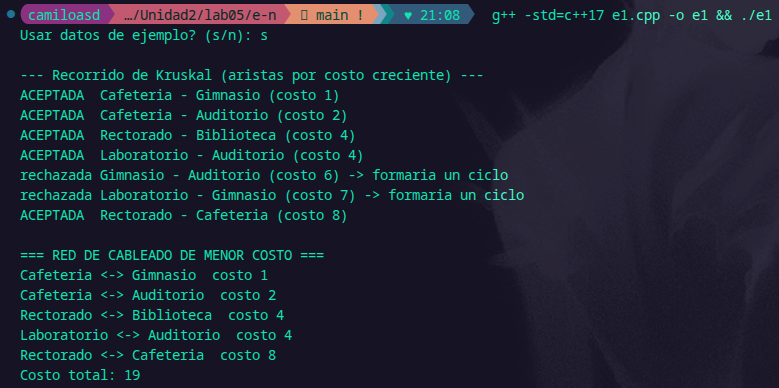
\includegraphics[width=0.8\textwidth]{../img/e1(1).png}
    \caption{Ejecución de e1.cpp con datos inicializados}
    \label{fig:e1}
\end{figure}

\begin{figure}[H]
    \centering
    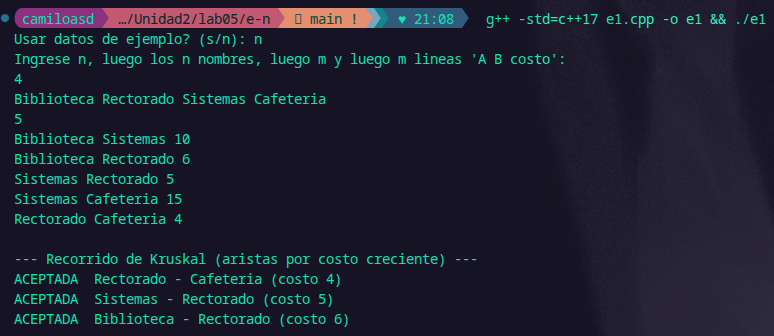
\includegraphics[width=0.8\textwidth]{../img/e1(2).png}
    \caption{Ejecución de e1.cpp con datos ingresados por el usuario}
    \label{fig:e1}
\end{figure}

\subsection{Ejercicio 2}

Implementa Prim con cola de prioridad y compara el árbol resultante (aristas y peso total) contra el obtenido con Kruskal sobre el mismo grafo.

\inputminted{cpp}{../e-n/e2.cpp}

\begin{itemize}
    \item Compara los algoritmos Kruskal y Prim que resuelven el MST, Kruskal ya lo vimos, por su parte, Prim no encuentra sino que construye el MST mediante una cola de prioridad (el min-heap), teóricamente esto lo hace uniendo la raiz con un nuevo vértice no visitado.
\end{itemize}

\begin{figure}[H]
    \centering
    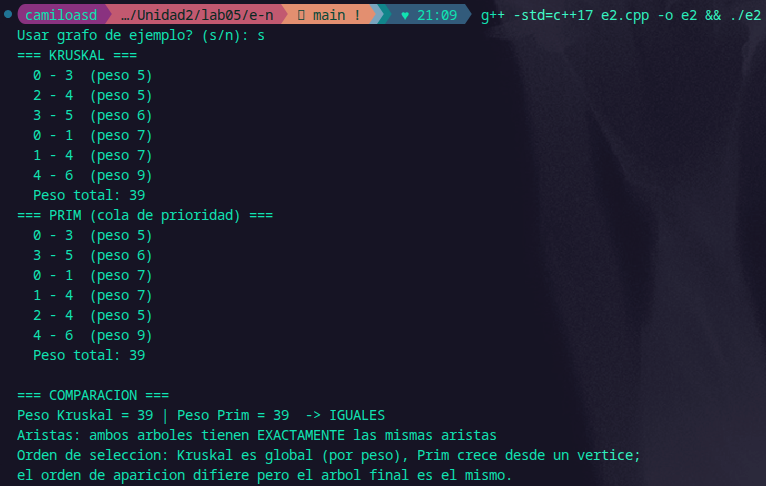
\includegraphics[width=0.8\textwidth]{../img/e2(1).png}
    \caption{Ejecución del e2.cpp con datos inicializados}
    \label{fig:e2}
\end{figure}

\begin{figure}[H]
    \centering
    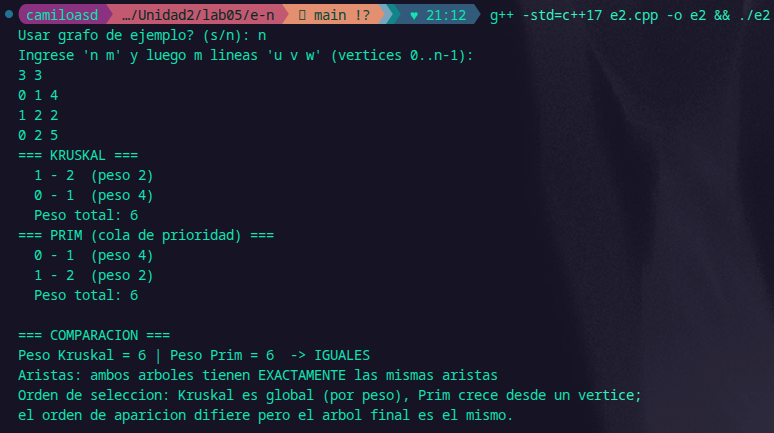
\includegraphics[width=0.8\textwidth]{../img/e2(2).png}
    \caption{Ejecución del e2.cpp con datos ingresados por el usuario}
    \label{fig:e2}
\end{figure}

\subsection{Ejercicio 3}

Implementa el algoritmo de Boruvka por rondas e imprime, en cada ronda, qué aristas se agregaron y cuántas componentes quedan, verificando que el resultado final coincide con el de Kruskal y Prim.

\inputminted{cpp}{../e-n/e3.cpp}

\begin{itemize}
    \item Se implementa el algoritmo de Boruvka, como es en la teoria, en cada ronda todas las componentes del grafo identifican simultaneamente su arista saliente menos costosa, su validacion se aprueba mediante Union-Find. Esto hace que en cada paso el número de componentes reduzca significativamente.
\end{itemize}

\begin{figure}[H]
    \centering
    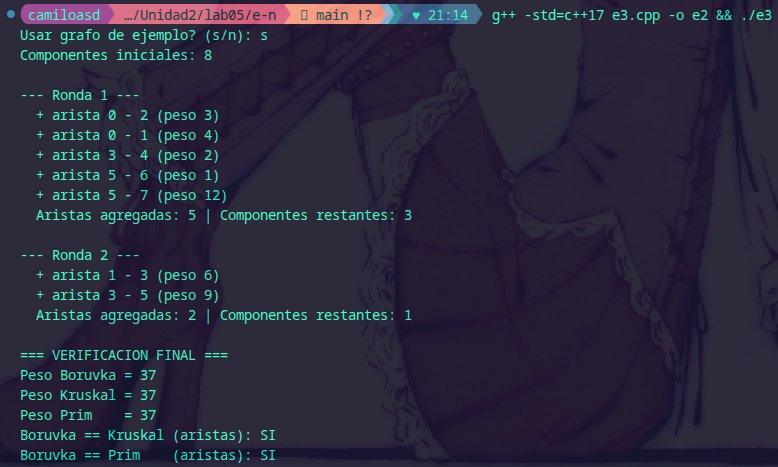
\includegraphics[width=0.8\textwidth]{../img/e3(1).png}
    \caption{Ejecución de e3.cpp con datos inicializados}
    \label{fig:e3}
\end{figure}

\begin{figure}[H]
    \centering
    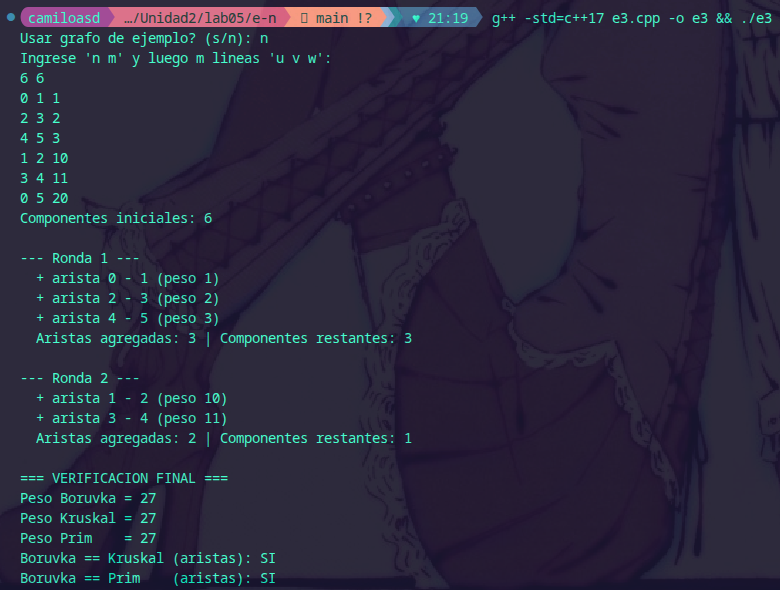
\includegraphics[width=0.8\textwidth]{../img/e3(2).png}
    \caption{Ejecución de e3.cpp con datos ingresados por el usuario}
    \label{fig:e3}
\end{figure}

\subsection{Ejercicio 4}

Genera grafos aleatorios densos y dispersos de distintos tamaños y compara los tiempos de ejecución de Kruskal y Prim, determinando en qué casos conviene usar cada uno.

\inputminted{cpp}{../e-n/e4.cpp}

\begin{itemize}
    \item Se comparan 3 algoritmos, Kruskal, Prim (con cola de prioridad) y Prim clasico (con matriz de adyacencia). Se genera grafos randoms de diferentes densidades, en grafos muy dispersos, es decir de baja densidad, Kruskal y Prim son mas eficientes por contraste: Prim clasico hace operaciones innecesarias basadas en el cuadrado del numero de vertices. Sin embargo, en grafos muy densos, Kruskal y Prim deben mantener un arbol muy grande, es costoso, Prim clasico no lidia con estos problemas. 
\end{itemize}

\begin{figure}[H]
    \centering
    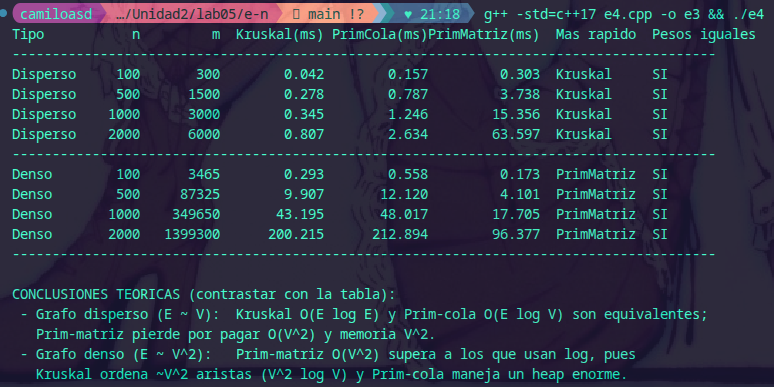
\includegraphics[width=0.8\textwidth]{../img/e4.png}
    \caption{Ejecución de e4.cpp}
    \label{fig:e4}
\end{figure}

\subsection{Ejercicio 5}

Modela una red de distribución eléctrica (o de agua) entre varias localidades como un grafo ponderado por costo de tendido, y calcula el costo mínimo de conectarlas todas usando Kruskal o Prim.

\inputminted{cpp}{../e-n/e5.cpp}

\begin{itemize}
    \item Se aplica Kruskal para resolver un problema de redes de distribución donde el costo por arista tiene un costo adicional de dinero, es por ello que se busca encontrar el MST. Primero calcula el costo financiero de cada tramo, luego con Union-Find se ordena de mayor a menor estos resultados y se aplica propiamente el algoritmo de Kruskal. Cuando se ejecuta simplemente calcula metricas del negocio, es una aplicación muy simple porque no toma en cuenta rutas alternativas en caso fallen algunas. 
\end{itemize}

\begin{figure}[H]
    \centering
    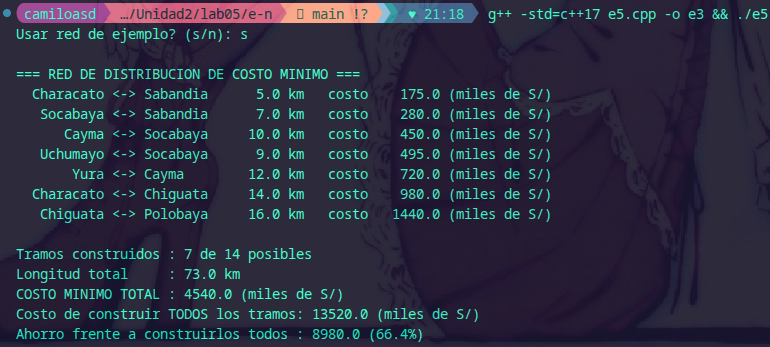
\includegraphics[width=0.8\textwidth]{../img/e5(1).png}
    \caption{Ejecución de e5.cpp con datos inicializados}
    \label{fig:e5}
\end{figure}

\begin{figure}[H]
    \centering
    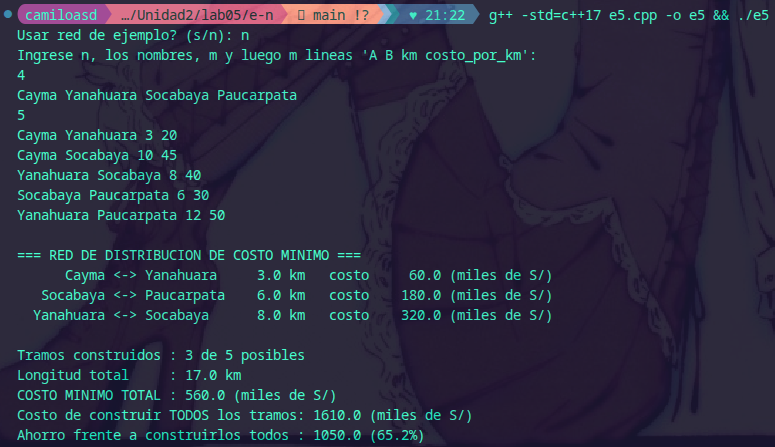
\includegraphics[width=0.8\textwidth]{../img/e5(2).png}
    \caption{Ejecución de e5.cpp con datos ingresados por el usuario}
    \label{fig:e5}
\end{figure}

\section{Cuestionario}

\begin{enumerate}
	\item ¿Por qué Kruskal necesita una estructura Union-Find, y qué problema resuelve la compresión de caminos dentro de esa estructura?

	Kruskal agrega las aristas de menor a mayor peso, pero antes de agregar una debe saber si sus dos extremos ya están conectados, porque si lo están, la arista cerraría un ciclo. Revisar eso recorriendo el grafo cada vez sería muy lento. Union-Find soluciona esto porque guarda los vértices en grupos y responde rápido a dos preguntas: ``¿estos dos vértices están en el mismo grupo?'' y ``junta estos dos grupos''.

	La compresión de caminos resuelve un problema de velocidad. Para saber a qué grupo pertenece un vértice hay que subir por sus padres hasta llegar a la raíz, y esa cadena puede ser larga. Con la compresión, todos los vértices por los que se pasó quedan apuntando directamente a la raíz, así que las siguientes búsquedas son casi inmediatas.

	\item ¿En qué se diferencia la estrategia de Prim de la de Kruskal, si ambos son algoritmos golosos?

	Los dos son golosos porque en cada paso eligen la arista más barata que no forma un ciclo. La diferencia está en cómo van construyendo el árbol.

	Kruskal revisa todas las aristas del grafo ordenadas por peso, y el resultado se va armando en varios pedazos que se unen poco a poco hasta formar un solo árbol. Prim, en cambio, hace crecer un único árbol desde un vértice inicial, y en cada paso elige la arista más barata que conecta ese árbol con un vértice que todavía no está dentro. Por eso Kruskal usa una lista de aristas ordenada junto con Union-Find, mientras que Prim usa una cola de prioridad.

	\item ¿Puede un grafo tener más de un árbol de expansión mínimo? ¿Bajo qué condición ocurre esto?

	Sí, puede ocurrir cuando hay aristas con el mismo peso, porque entonces existen varias formas de elegir y todas dan el mismo costo total. Si todos los pesos del grafo son distintos, el árbol de expansión mínimo es único.

	Por ejemplo, en un triángulo donde las tres aristas pesan 1, se puede dejar fuera cualquiera de ellas, y así hay tres árboles posibles. Los tres pesan 2. Lo que nunca cambia es el peso total, que siempre es el mínimo.

	\item ¿Por qué se dice que Boruvka es un algoritmo naturalmente paralelizable?

	En cada ronda de Boruvka, cada componente elige su arista más barata sin necesitar saber qué están eligiendo las demás. Como esas decisiones son independientes entre sí, se pueden repartir entre varios procesadores o hilos y hacerlas al mismo tiempo.

	Kruskal y Prim, en cambio, avanzan paso a paso, y cada decisión depende de lo que se decidió antes. Además, Boruvka necesita pocas rondas (como máximo $\log_2 n$), porque en cada una el número de componentes se reduce al menos a la mitad.

	\item ¿Qué diferencia fundamental existe entre el problema del árbol de expansión mínimo y el problema del camino más corto visto en el Laboratorio 4?

	El árbol de expansión mínimo busca conectar todos los vértices del grafo gastando lo menos posible en total, como cuando se quiere cablear todos los edificios de una universidad. El camino más corto, en cambio, busca la mejor ruta entre un origen y un destino específicos, como cuando se quiere ir de un punto a otro recorriendo la menor distancia.

	Los resultados no son equivalentes. Si tenemos los vértices A, B y C con las aristas A--B de peso 1, B--C de peso 1 y A--C de peso 1.5, el árbol de expansión mínimo usa A--B y B--C, y para ir de A a C dentro del árbol hay que recorrer 2. Sin embargo, el camino más corto de A a C es la arista directa, que pesa 1.5.
	\end{enumerate}

\section{Conclusiones}

\begin{itemize}
	\item Se implementaron tres algoritmos para encontrar el árbol de expansión mínimo: Kruskal (con Union-Find y compresión de caminos), Prim (con cola de prioridad) y Boruvka (por rondas). Los tres obtuvieron el mismo peso total sobre el mismo grafo, lo que confirma que el resultado mínimo es único aunque cada algoritmo llegue a él por un camino distinto.

	\item Union-Find es lo que hace eficiente a Kruskal, ya que permite detectar ciclos casi de inmediato. La compresión de caminos y la unión por rango evitan que los grupos se vuelvan cadenas largas y lentas de recorrer.

	\item Prim y Kruskal no siempre rinden igual. Kruskal depende de ordenar todas las aristas, por lo que se comporta bien en grafos con pocas conexiones, mientras que Prim suele convenir más cuando el grafo tiene muchas aristas, ya que solo trabaja con las que salen del árbol que va construyendo.

	\item Boruvka destaca porque sus decisiones en cada ronda son independientes, lo que lo hace muy adecuado para trabajar en paralelo. Además, mostrar las aristas agregadas y las componentes restantes en cada ronda ayudó a entender cómo el grafo se va uniendo poco a poco.

	\item Estos algoritmos tienen aplicaciones reales. Al modelar una red de distribución eléctrica entre localidades, se comprobó que construir solo los tramos del árbol de expansión mínimo permite conectar todas las localidades con un costo mucho menor que construir todos los tramos posibles.

\end{itemize}
% Pendiente de completar.

	%\begin{itemize}	
	%	\item Se creo el archivo \textbf{.gitignore} para no considerar los archivos %\textbf{*.class} que son innecesarios hacer seguimiento.
	%\end{itemize}
    
%\clearpage
%\bibliographystyle{apalike}
%\bibliographystyle{IEEEtranN}
%\bibliography{bibliography}
			
\end{document}\noindent\textbf{Enunciado:}
